\chapter{ทฤษฎีและงานวิจัยที่เกี่ยวข้อง}
\section{ทฤษฎีที่เกี่ยวข้อง}
\subsection{ระบบการตรวจจับท่าทางของมนุษย์ (Pose Estimation)}
ระบบการตรวจจับท่าทางของมนุษย์ หรือการทำ Pose Estimation คือระบบที่จะทำการตรวจจับตัวบุคคลในรูปภาพ หรือวิดีโอ แล้วจึงทำการอนุมานจุดต่าง ๆ บนตัวบุคคลในรูปภาพหรือวิดีโอนั้น ๆ ซึ่งกระบวนการทำงานและสถาปัตยกรรมของแต่ละโมเดลจะมีความแตกต่างกันออกไป
\\\indent
จากการศึกษาโมเดล Pose Estimation ที่จะนำมาใช้กับโครงงาน พบว่าในแต่ละโมเดลจะมีขั้นตอนและเทคนิคการปรับปรุงประสิทธิภาพที่แตกต่างกันไป เพื่อให้สามารถตรวจจับได้มีประสิทธิภาพได้มากขึ้น เช่น ในโมเดล BlazePose การทำงานจะมีทั้งหมด 2 ขั้นตอน ดังนี้

\begin{enumerate}
    \item ขั้นตอนการตรวจจับตัวบุคคลในเฟรมของรูปภาพหรือวิดีโอ \\ในขั้นตอนนี้โมเดลจะทำการตรวจจับตัวบุคคลโดยดูจากส่วนที่ไม่เคลื่อนไหวมากในตัวบุคคล เช่น ใบหน้าหรือลำตัว ซึ่งโมเดลนี้ได้สมมติว่าในเฟรมนั้น ๆ จะต้องมีหัวของบุคคลนั้น ๆ อยู่ตลอดเวลาจึงจะถือว่ามีบุคคลอยู่ในเฟรม
    \item ขั้นตอนการอนุมานจุดต่าง ๆ บนตัวบุคคล\\เมื่อได้ตำแหน่งของตัวบุคคลในรูปภาพเรียบร้อยแล้ว โดยใช้ Neural Network ของโมเดล ซึ่งจะทำให้ได้ค่าพิกัดของจุดต่าง ๆ บนร่างกาย
\end{enumerate}

\subsection{ระบบการตรวจสอบความถูกต้องของท่าทาง (Pose Classification)}
ระบบการตรวจสอบความถูกต้องของท่าทาง หรือการทำ Pose Classification เป็นระบบที่มีความสำคัญในโครงงานนี้ ซึ่งจะได้นำไปใช้ในระบบการให้คำแนะนำท่าทางการออกกำลังกายของผู้ใช้ ซึ่งใน API ของ ML Kit มีการใช้อัลกอริทึม K-NN (K-Nearest Neighbors) ในการวิเคราะห์ท่าทางและนับจำนวนครั้งในการทำท่าทาง โดยอัลกอริทึมจะกำหนดคลาสของ Object โดยพิจารณาจากตัวอย่าง Training Set ที่ใกล้เคียงที่สุด
\\\indent
จากการศึกษาการทำ Pose Classification จะมีขั้นตอนการพัฒนาดังนี้
\begin{enumerate}
    \item ทำการเก็บชุดภาพตัวอย่างของท่าทางการออกกำลังกาย (Training Set) จากหลากหลายแหล่งที่มา, มุมกล้อง, สภาพแวดล้อม, รูปร่างร่างกาย, รูปแบบการออกกำลังกาย โดยเก็บภาพตัวอย่างในแต่ละท่าทางไม่ต่ำกว่า 100 ภาพต่อท่าทาง
    \item ทำการรันระบบตรวจจับท่าทางในชุดภาพตัวอย่างของท่าทางการออกกำลังกาย (Training Set) ได้ผลลัพธ์เป็นค่าพิกัดของจุดต่าง ๆ บนร่างกาย จากนั้นนำพิกัดระหว่างคู่ของข้อต่อมาคำนวณหาระยะทางเพื่อนำมาหาท่าทางที่
    ใกล้เคียงกับตัวอย่างมากที่สุดโดยใช้อัลกอริทึม K-NN
\end{enumerate}


\subsection{NoSQL}
NoSQL หรือ Not Only SQL เป็น Unstructured ของ Database แบบ SQL เป็นแนวทางการแก้ไขปัญหาของ Database ที่มีข้อมูลขนาดใหญ่และไม่มีรูปแบบที่ชัดเจน โดยไม่จำเป็นต้องเก็บข้อมูลแบบ Table เดียวที่ต้องมีข้อมูลเหมือนกันทั้งหมดในหนึ่ง Table แต่สามารถจัดเก็บข้อมูลได้หลายรูปแบบ

\section{งานวิจัยที่เกี่ยวข้อง}

\subsection{Pose Trainer: Correcting Exercise Posture using Pose Estimation}
งานวิจัยที่เกี่ยวข้องกับการวิเคราะห์ความถูกต้องของท่าทางในการออกกำลังกาย โดยการตรวจจับท่าทางการออกกำลังกายของผู้ใช้ ให้คำแนะนำส่วนบุคคลและมีรายละเอียดในการแนะนำผู้ใช้ว่าสามารถปรับปรุงการจัดระเบียบร่างกายของตนเองให้ดีขึ้นได้อย่างไร งานวิจัย Pose Trainer ทำงานบนการฝึกออกกำลังกาย 4 ท่าทางพื้นฐานและรองรับคอมพิวเตอร์ Windows หรือ Linux ที่มีหน่วยประมวลผลด้านกราฟิก
\subsubsection{Pipeline ของระบบ Pose Trainer}
\begin{figure}
    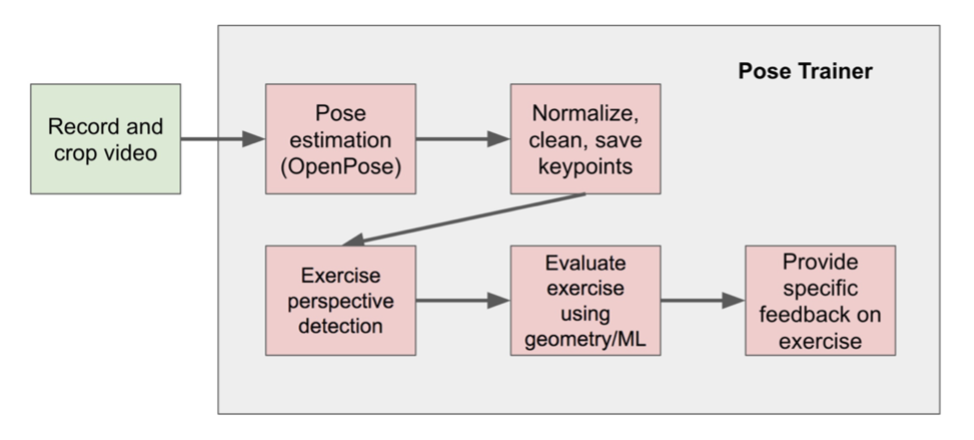
\includegraphics[width=10cm]{PoseTrainer Pipeline}
    \caption{แสดง Pipeline ของระบบ Pose Trainer}
\end{figure}

\begin{enumerate}
    \item ขั้นตอนการบันทึกวิดีโอของผู้ใช้\\
    ในขั้นตอนแรกจะเป็นการให้ผู้ใช้บันทึกวิดีโอการออกกำลังกายของตนเอง ซึ่งผู้ใช้สามารถบันทึกจากมุมใด ๆ ก็ได้ และจะไม่มีข้อจำกัดในเรื่องประเภทของกล้อง และระยะห่างของกล้อง แต่ผู้ใช้จำเป็นต้องถ่ายให้เห็นลำตัวในขณะออกกำลังกาย
    \item Pose Estimator\\
    สำหรับการตรวจจับท่าทาง ทางผู้วิจัยได้ใช้ Deep Convolutional Neural Networks (CNNs) ในการจำแนกรูปภาพ RGB ซึ่งในงานวิจัยนี้จะใช้ OpenPose เป็นโมเดลสำหรับการตรวจจับท่าทาง ซึ่งสาเหตุที่ทางผู้วิจัยได้เลือกใช้โมเดลนี้ เพราะว่า OpenPose เป็นโมเดลที่มีความแม่นยำสูงและมีประสิทธิภาพ ในขณะที่ยังสามารถต่อยอดเป็นการตรวจจับท่าทางหลาย ๆ คนพร้อมกันได้โดยที่ไม่ได้มีผลกระทบต่อประสิทธิภาพของระบบ
    \item Keypoint Normalization\\
    ผู้วิจัยได้พัฒนา parser ขึ้นเพื่อใช้กับค่า keypoint ที่ได้รับมาจากขั้นตอนที่แล้ว ในขั้นแรกจะเป็นการอ่านค่า keypoint ทั้งหมดที่ได้รับ และแยก keypoint ที่ได้ออกเป็น Part object ซึ่งจะเก็บค่า x, y และค่า confidence ของแต่ละ keypoint จากนั้นระบบจะทำการรวมแต่ละ Part object และสร้างเป็น skeleton ของตัวคนที่ได้ predict ขึ้น จากนั้นตัวระบบจะ normalize ข้อมูลท่าทางโดยยึดตามความยาวของลำตัวเป็นหน่วย pixel ซึ่งจะคำนวณได้จากค่าเฉลี่ยของความห่างระหว่าง keypoint ของส่วนคอ กับ keypoint ของส่วนสะโพก
    \item Perspective Detection\\
    ทางผู้วิจัยได้ทำการแก้ไขความกำกวมของมุมกล้องในหลาย ๆ ท่าทางการออกกำลังกาย เช่นในท่า bicep curl จะสามารถใช้แขนข้างใดก็ได้ ถ้ามุมกล้องเป็นมุมด้านข้างจะทำให้เกิดความกำกวมขึ้น ทางผู้วิจัยจึงแก้ไขโดยการวัดว่า keypoint ด้านไหนที่เห็นมากที่สุดในของทั้งวิดีโอ
    \item Geometry Evaluation\\
    ต่อไปจะทำการคำนวณ body vector จาก keypoint ที่สนใจ และได้ทำการออกแบบ geometric heuristics เพื่อนำมาวัดผลใน body vector เพื่อทำการวัดผลการออกกำลังกาย
    \item Machine Learning Evaluation\\
    การวัดผลท่าทางการออกกำลังกายอีกรูปแบบหนึ่งที่ผู้วิจัยได้นำมาใช้คือการนำ machine learning มาปรับใช้ โดยจะใช้ dynamic time warping (DWT) และ nearest neighbor classifier
\end{enumerate}

\subsubsection{ผลจากการทดลอง}
ทางผู้วิจัยได้ทำการทดลองกับ 4 ท่าทางการออกกำลังกาย คือ bicep curl, front raise, shoulder shrug, standing shoulder press ซึ่งในแต่ละท่าทางจะมีการใช้ทั้งเทคนิค geometry evaluation และ machine learning ในการวัดผลท่าทางการออกกำลังกาย
\begin{enumerate}
    \item Bicep Curl\\
    ท่า Bicep Curl ที่นำมาทดลอง ใน algorithm แบบ geometric ทางผู้วิจัยได้ใช้มุมระหว่างแขนท่อนบนและลำตัว (เพื่อวัดว่าผู้ใช้ได้หมุนข้อแขนระหว่างการออกกำลังกายหรือไม่) และ วัดมุมระหว่างแขนท่อนบนที่ทำมุมกับแขนท่อนล่าง (เพื่อวัดว่าผู้ใช้ยกได้สูงเท่าใด) จากการทดลองพบว่า algorithm นี้สามารถจำแนกการออกกำลังกายที่ถูกต้องได้ทั้งหมด และ วิดีโอที่ออกกำลังกายที่ผิดจำนวน 8\% ได้ถูกจำแนกโดย algorithm นี้ว่าเป็นการออกกำลังกายที่ไม่ถูกต้อง สำหรับ algorithm ที่ใช้ machine learning ผู้วิจัยได้แบ่ง dataset จำนวน 16 วิดีโอออกเป็น training set จำนวน 9 examples และ test set จำนวน 7 examples ซึ่งผลลัพธ์ของ DTW จะได้ค่า F1 อยู่ที่ 0.85
    \item Front Raise\\
    ท่า Front Raise เมื่อใช้ geometric algorithm จะทำการวัดการเคลื่อนที่ของหลังผู้ใช้ในแนวราบ และวัดมุมที่มากที่สุดระหว่างลำตัวและแขน สำหรับ algorithm ที่ใช้ machine learning จะแบ่ง dataset จำนวน 28 วิดีโอออกเป็น training set จำนวน 16 examples และ test set จำนวน 12 examples ซึ่งได้คะแนน F1 เป็น 1.0
    \item Shoulder Shrug\\
    ในท่า Shoulder Shrug เมื่อใช้ geometric algorithm จะวัดความเคลื่อนไหวของไหล่ผู้ใช้ และวัดมุมระหว่างแขนท่อนบนกับท่อนล่าง สำหรับ machine learning algorithm จะแบ่ง dataset จำนวน 32 วิดีโอออกเป็น training set จำนวน 19 examples และ test set จำนวน 13 examples ซึ่งได้คะแนน F1 เป็น 0.85
    \item Shoulder Press\\
    ในท่า Shoulder Press เมื่อใช้ geometric algorithm จะวัดการเคลื่อนที่ของหลังผู้ใช้โดยการนำ keypoint ของคอและสะโพกมาใช้, วัดการเคลื่อนที่ของแขนโดยใช้ keypoint ของข้อศอกและคอ และวัดมุมองศาสูงสุดที่ทำมุมระหว่างแขนท่อนบนกับท่อนล่าง สำหรับ machine learning algorithm จะแบ่ง dataset จำนวน 36 วิดีโอออกเป็น training set จำนวน 21 examples และ test set จำนวน 15 examples ซึ่งได้คะแนน F1 เป็น 0.73
\end{enumerate}

\begin{figure}
    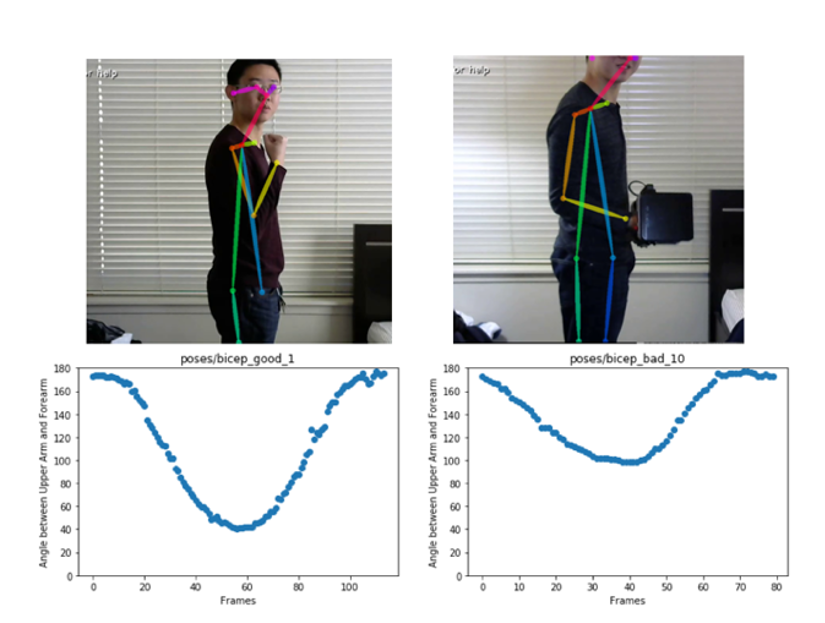
\includegraphics[width=10cm]{Bicep Curl}
    \caption{แสดงรูปภาพและกราฟองศาระหว่างแขนท่อนบนและท่อนล่างของการออกกำลังกายท่า Bicep Curl}
\end{figure}

\begin{figure}
    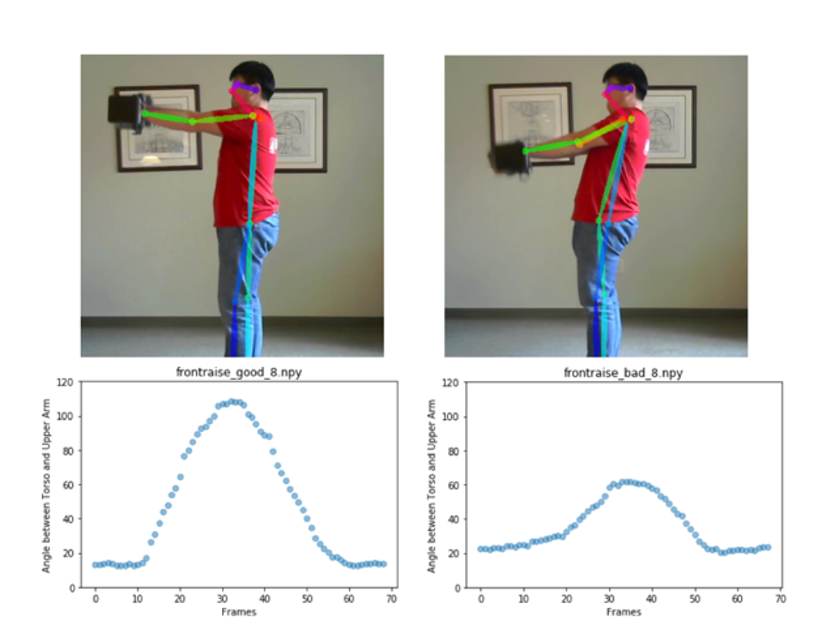
\includegraphics[width=10cm]{Front Raise}
    \caption{แสดงรูปภาพและกราฟองศาระหว่างแขนท่อนบนกับลำตัวของการออกกำลังกายท่า Front Raise}
\end{figure}

\begin{figure}
    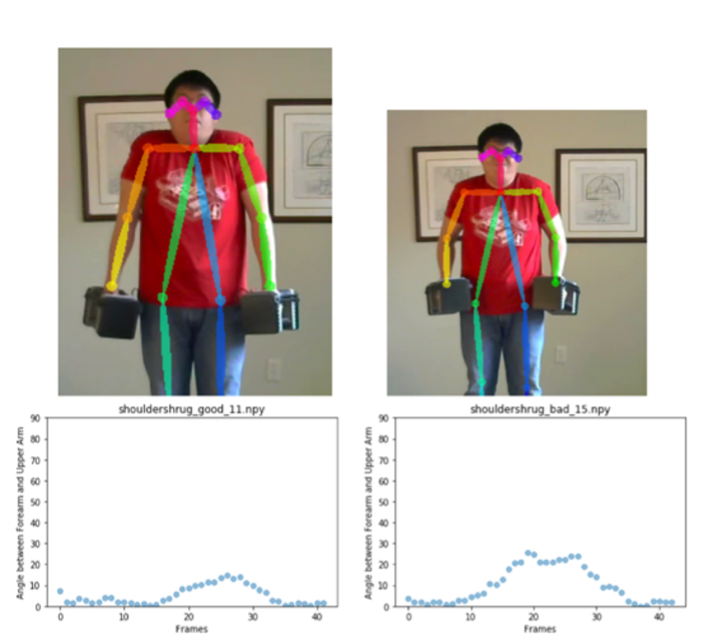
\includegraphics[width=10cm]{Shoulder Shrug}
    \caption{แสดงรูปภาพและกราฟองศาระหว่างแขนท่อนบนกับแขนท่อนล่างของการออกกำลังกายท่า Shoulder Shrug}
\end{figure}

\begin{figure}
    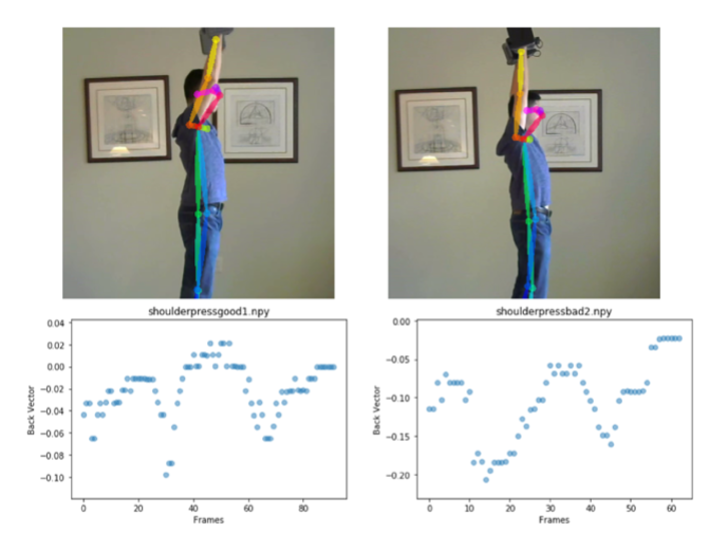
\includegraphics[width=10cm]{Shoulder Press}
    \caption{แสดงรูปภาพและกราฟการเคลื่อนที่ของหลังของการออกกำลังกายท่า Shoulder Press}
\end{figure}

\begin{figure}
    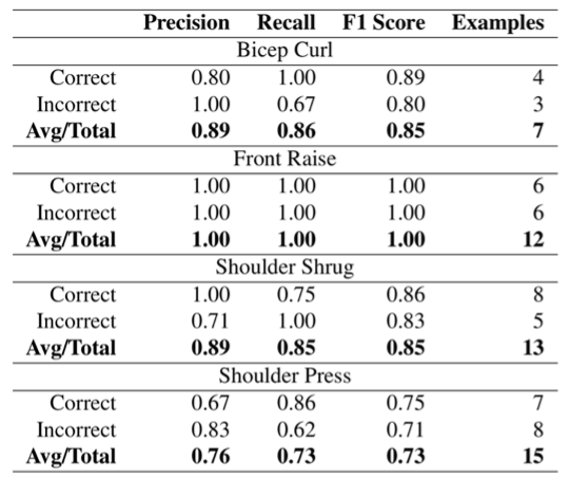
\includegraphics[width=10cm]{Post Trainer Performance}
    \caption{ตารางประสิทธิภาพและคะแนนความถูกต้องของ Machine Learning Algorithm}
\end{figure}

\subsection{Virtual Trainer with Real-Time Feedback using Kinect Sensor}
งานวิจัยการใช้ Kinect Sensor มาเป็นผู้ฝึกสอนเสมือนจริงพร้อมข้อเสนอแนะในการออกกำลังกายแบบเรียลไทม์
พร้อมมีระบบการให้คะแนนผู้ใช้เพื่อให้ผู้ใช้ได้ปรับท่าทางการออกกำลังกายได้อย่างถูกต้อง
โดยประสิทธิภาพของระบบได้ถูกประเมินโดยผู้ใช้แต่ละบุคคลที่ความแม่นยำ 96\%
โดยมี Flow Diagram ของงานวิจัยเป็นดังนี้


\begin{figure}
    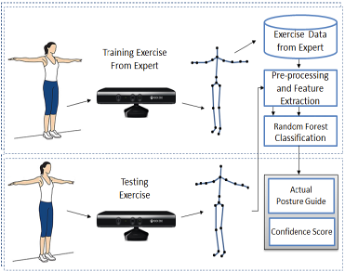
\includegraphics[width=10cm]{Virtual Trainer Flow Diagram}
    \caption{Flow Diagram ของงานวิจัย Virtual Trainer with Real-Time Feedback using Kinect Sensor}
\end{figure}

\subsubsection{หลักการที่เกี่ยวข้องในงานวิจัย}

\begin{enumerate}
    \item ในการทำงานเริ่มต้นจะแสดงระบบโต้ตอบเป็นโมเดล 3 มิติให้ผู้ใช้ได้ทำท่าทางตาม จากนั้นระบบจะแสดงคะแนนเพื่อบ่งบอกความถูกต้องของท่าทางที่ผู้ใช้ได้ออก จากการคำนวณ Random Forest (RF) Classifier ของท่าทางที่ได้ทำการฝึกไว้ และนำมาคำนวณหาค่าความเชื่อมั่น (Confidence Score)
    \item โดยก่อนที่จะทำการ Classification จะมีการทำการแปลงโครงร่างกาย 3 มิติ โดยใช้จุดกำเนิดร่วมกัน คือ
    \begin{itemize}
        \item Joint Selection: มีการเลือกข้อต่อที่ใช้เพียง 12 จุด ($J_k,k = 1, 2, 3, ..., 12$) เพื่อลดความซ้ำซ้อน และสิ่งรบกวนในบางจุดโดยใช้อัลกอริทึม evolutionary algorithm แสดงดังรูป (a)
        \item 	Angular Features: จาก Joint Selection 12 จุด ได้เป็น 8 เชิงมุม ($J_i,i = 1, 2, 3, ..., 8$) นำมาคำนวณหามุม cosine ระหว่าง 2 เวกเตอร์โดยใช้สมการ (\ref{eq:cosine}), โดยที่เวกเตอร์ X และ Y เกิดขึ้นโดยใช้ 3 ข้อต่อ แสดงดังรูป (b) และเซตของ Final Feature ($F_T$) จะประกอบด้วยเซตของ Joint Selection และ Angular Features ตามสมการ (\ref{eq:angularFeatures}) ประกอบด้วย 44 มิติ
    \end{itemize}

    \begin{equation}
        A_i = cos\alpha = \frac{\vec{X}\vec{Y}}{|X||Y|}
        \label{eq:cosine}
    \end{equation}

    \begin{equation}
        F_T = \{J_k, A_i\}
        \label{eq:angularFeatures}
    \end{equation}


    \begin{figure}
        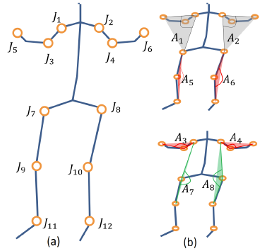
\includegraphics[width=7cm]{SelectedJointsAndAngularFeatures}
        \caption{แสดง (a) Selected joints (b) Angular features}
    \end{figure}

    \item การทำ Classification โดยการใช้หลักการ Random Forest (RF) และมีการใช้ GINI Index (GI) ในการแยกการเลือกที่วัดความไม่บริสุทธิ์ของตัวอย่างข้อมูลในคลาส โดยกำหนดให้ node t และ GI สามารถคำนวณได้โดยใช้สมการ (\ref{eq:Posterior probability}) จากนั้นตัวอย่างทดสอบจะส่งต่อไปยัง Leaf node และการ Classification จะดำเนินการโดยใช้ Posterior probability
    
    \begin{equation}
        GI(t) = 1-\sum_{x=1}^{Q}p^2(x|t)
        \label{eq:Posterior probability}
    \end{equation}
    จากสมการ (\ref{eq:Posterior probability}) $p(x│t),{x=1,2,...Q}$ หมายถึงความน่าจะเป็นของคลาสโดยประมาณสำหรับจำนวนคลาส $Q$
\end{enumerate}

แหล่งข้อมูลที่นำมาใช้ได้เลือกท่าทางการออกกำลังกายแบบพื้นฐาน 9 ท่าทาง และได้ลงทะเบียนอาสาสมัครจำนวน 10 คนมาทำการเก็บข้อมูลท่าทางการออกกำลังกาย มีการเก็บข้อมูลคนละ 9 ท่าทาง จึงได้ทั้งหมด 900 ตัวอย่าง ซึ่งพบความหลากหลายในการออกกำลังกายท่าเดียวกันแต่ออกท่าทางแตกต่างกัน
\\\indent
มีการแบ่งการเก็บ Training set และ Test set จากการลงทะเบียนอาสาสมัครทั้งหมด 10 คนที่ทำการเก็บข้อมูลท่าทางการออกกำลังกาย มีการเก็บ Training set จำนวน 4 จาก 10 คนผู้ซึ่งเป็นผู้เชี่ยวชาญด้านการออกกำลังกาย และเก็บ Test set จำนวน 6 คนที่เหลือ
\\\indent
มีการทำการเปรียบเทียบกับวิธีการอื่นที่เกี่ยวข้อง โดยใช้อุปกรณ์ Kinect เช่นเดียวกัน โดยเก็บข้อมูลจำนวน 6 คน และมีท่าทางการออกกำลังกายที่แตกต่างกัน 5 ท่าทาง  และเป็นการประมวลผลแบบ Real-time จากการเปรียบเทียบงานวิจัยนี้กับงานวิจัยที่เกี่ยวข้องนั้นพบว่างานวิจัยนี้ได้ผลความแม่นยำที่สูงกว่างานวิจัยที่นำมาเปรียบเทียบ ดังรูปที่ \ref{fig:Kinect-Compare}

\begin{figure}
    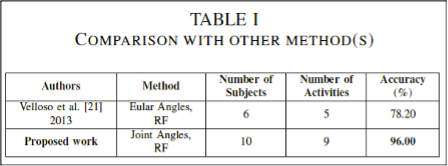
\includegraphics[height=3cm]{Kinect-Compare}
    \caption{ภาพตารางการเปรียบเทียบกับวิธีการอื่น}
    \label{fig:Kinect-Compare}
\end{figure}


\begin{table}
    \caption{ตารางเปรียบเทียบความแตกต่างของงานวิจัย}
    \begin{tabularx}{\textwidth}{ | p{4.45cm} | X | X | }
        \hline
        \textbf{หัวข้อ / งานวิจัย} & \textbf{Pose Trainer} & \textbf{Virtual Trainer with Real-Time Feedback using Kinect Sensor}\\\hline
        เทคนิคตรวจจับท่าทางที่ใช้ & ใช้โมเดล OpenPose & ใช้เทคนิค Joint Angles, Depth Sensor\\\hline
        ผลลัพธ์การตรวจจับ & ได้ผลลัพธ์ออกมาเป็น keypoint ตามจุดต่าง ๆ บนร่างกาย & ได้ผลลัพธ์เป็น keypoint ตามจุดต่าง ๆ ของร่างกาย\\\hline
        เทคนิคการวิเคราะห์ความถูกต้องของท่าทาง & Geometric, Machine Learning & Random Forest Classifier\\\hline
        ผลลัพธ์ที่ต้องการได้รับ & คำแนะนำของท่าทางการออกกำลังกาย & คะแนนความถูกต้องของท่าทาง\\\hline
        ข้อมูลที่นำมาใช้ & วิดีโอการออกกำลังกาย & ข้อมูลวิดีโอจากการเก็บข้อมูลจากอาสาสมัคร\\\hline
        รูปแบบการแบ่งข้อมูล & ขึ้นอยู่กับแต่ละท่าทาง & Training Set 4 คน, Test Set 6 คน\\\hline
        ประสิทธิภาพเชิงความถูกต้อง & ค่า F1 เท่ากับ 0.73 – 1.00 ขึ้นอยู่กับแต่ละท่าทาง & ค่า Accuracy เท่ากับ 96\%\\\hline
        จุดเด่น & เป็นระบบที่ใช้เพียงกล้องในการถ่ายวิดีโอการออกกำลังกาย  & เป็นระบบที่มีความแม่นยำสูง, ระบบเป็นแบบ Realtime\\\hline
        จุดด้อย & ระบบมีความแม่นยำน้อยกว่าอีกระบบหนึ่ง & จำเป็นต้องใช้ Kinect Sensor เพื่อใช้งานระบบนี้\\\hline
    \end{tabularx}
\end{table}
\clearpage

\section{เครื่องมือที่เกี่ยวข้อง}
\subsection{MongoDB}
MongoDB เป็น Open-Source Document Database โดยเป็นฐานข้อมูลแบบ NoSQL มีการเก็บข้อมูลเป็นแบบ JavaScript Object Notation (JSON) มีการบันทึกข้อมูลทุก ๆ Record เรียกว่า Document ซึ่งจะเก็บค่าเป็น Key และ Value และการเก็บข้อมูล Document จะถูกเก็บไว้ใน Collections (เปรียบเทียบได้กับ Table ใน Relational Database) แต่แตกต่างกันที่ Collection ไม่จำเป็นที่จะต้องมี Schema เหมือนกันก็สามารถบันทึกข้อมูลได้

% TODO: Change Pixlated MongoDB Picture
\begin{figure}
    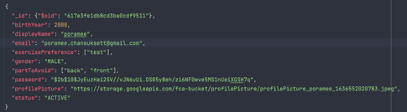
\includegraphics{mongodb example}
    \caption{ตัวอย่างโครงสร้างข้อมูลที่เก็บใน MongoDB}
\end{figure}

\subsection{Google Cloud Platform}
Google Cloud Platform คือ บริการในรูปแบบ Cloud ซึ่งจะมีผลิตภัณฑ์ที่หลากหลายโดยจะเน้นไปที่การประมวลผลแบบ Cloud และ บริการจัดเก็บไฟล์ โดยในโครงงานนี้จะใช้ผลิตภัณฑ์ 2 ตัวใน Google Cloud Platform คือ Google Cloud Functions และ Google Cloud Storage
\\\indent
Google Cloud Functions คือ บริการประมวลผลฟังก์ชันแบบไร้เซิร์ฟเวอร์ (Serverless) ซึ่งสามารถเรียกใช้ได้ผ่าน Trigger ต่าง ๆ ที่ได้กำหนดไว้ โดยในโครงงานนี้จะนำ Google Cloud Functions มาใช้สำหรับการทำ API เพื่อติดต่อกับ database และจะสามารถเรียกใช้ได้ผ่าน HTTP Request โดยเมื่อได้พัฒนา API บนเครื่องคอมพิวเตอร์โดยใช้ Node.js และ Push ขึ้น GitHub เรียบร้อยแล้ว ในโครงงานนี้จะเรียกใช้ GitHub Actions ในการ deploy ขึ้นไปยัง Google Cloud Functions โดยอัตโนมัติ
\\\indent
Google Cloud Storage คือ บริการจัดเก็บไฟล์ในรูปแบบออนไลน์ โดยใน Google Cloud Storage จะจัดเก็บในรูปแบบ object ซึ่ง object นี้จะเป็นชุดข้อมูลที่จะประกอบไปด้วยไฟล์เพียงไฟล์เดียว และ object นี้จะถูกจัดเก็บรวมกันใน container หนึ่งที่จะเรียกว่า bucket การใช้ Google Cloud Storage มีข้อดีคือสามารถตั้งค่าสิทธิ์ในการเข้าถึงไฟล์ (Permission) ได้อย่างละเอียด และสามารถใช้งานร่วมกับ Node.js ได้ดี โดยในโครงงานนี้จะใช้ Google Cloud Storage เก็บข้อมูลรูปภาพของผู้ใช้ และไฟล์คอร์สข้อมูลท่าทางการออกกำลังกาย ซึ่งในแต่ละไฟล์จะมี URL ที่สามารถเข้าถึงได้กำกับไว้ โดยที่จะจัดเก็บ URL นี้เป็น String ใน database ต่อไป

\subsection{MongoDB Atlas}
MongoDB Atlas เป็นผู้ให้บริการ MongoDB บนระบบ Cloud (MongoDB as a service) ที่ให้บริการโดยผู้พัฒนา MongoDB โดยตรง ซึ่งจะสามารถเลือก Cloud Provider สำหรับการวางระบบได้ โดยบริการนี้จะเข้ามาช่วยดูแลเรื่องการกำหนดค่าต่าง ๆ ทำให้ง่ายต่อการใช้งาน

\subsection{Node.js}
Node.js คือ Runtime Environment สำหรับฝั่ง Server ซึ่งเขียนจะด้วยภาษา JavaScript และสามารถลง Library หรือ Package อื่น ๆ เพิ่มเติมได้ ผ่าน NPM (Node Package Manager) โดยในโครงงานนี้จะนำ Node.js มาใช้งานสำหรับการพัฒนา API ซึ่งจะถูกเรียกใช้โดยแอปพลิเคชัน และจะ Deploy โดยใช้ Google Cloud Functions

\subsection{Express.js}
Express.js เป็น Web Framework ที่ใช้สำหรับการพัฒนาเว็บแอปพลิเคชันฝั่ง Backend โดย Framework นี้จะมีฟีเจอร์ที่เข้ามาช่วยในการพัฒนา API ของโครงงาน เช่น การจัดการ Routing, มีการสนับสนุน Middleware, การจัดการ Request และ Response เป็นต้น ทำให้การพัฒนาสะดวกและรวดเร็วขึ้น

\subsection{GitHub Actions}
GitHub Actions เป็นเครื่องมือของ GitHub ที่จะช่วยลดขั้นตอนการ Test และ Deploy โดยการเขียน Script เพื่อให้ GitHub Actions ทำงานให้อัตโนมัติ ซึ่งในโครงงานนี้จะนำมาใช้ในการทำ Automatic Testing และ Deploy โดยอัตโนมัติของทางฝั่ง Backend ซึ่งจะสามารถเขียน Script ให้ GitHub Actions ทำการ Build โปรแกรมและ Test อัตโนมัติเมื่อมีการ Push หรือ Merge Source Code เข้าสู่ branch ที่กำหนดไว้ได้

\subsection{ML Kit}
ML Kit เป็น Software Development Kit (SDK) สำหรับ Machine Learning บนระบบปฏิบัติการ Android และ iOS ประกอบด้วยสองส่วนหลัก คือ Base APIs และ Custom model ซึ่งสามารถใช้งานได้ทั้งแบบ Offline (On-device) และ Online (Google Cloud AI)
\\\indent
โดยในส่วนของแอปพลิเคชันที่จะนำมาใช้ในการพัฒนาโครงงานนี้คือในส่วนของ Pose Detection หรือการตรวจจับร่างกายซึ่งสามารถตรวจจับท่าทางของร่างกายแบบ Realtime จากวิดีโอต่อเนื่องหรือภาพนิ่ง โดยสามารถระบุจุดเป็น Landmark ต่าง ๆ ทั่วร่างกายทั้งหมด 33 จุด โดยจะนำค่าตำแหน่งต่าง ๆ ที่ได้รับมาวิเคราะห์หาท่าทางที่ต่างกันได้ เช่นการนำพิกัดที่แตกต่างกันมาใช้ในการนับจำนวนครั้งของการวิดพื้น หรือการนำค่าพิกัดที่แตกต่างกันมาเปรียบเทียบท่าทางการออกกำลังกายของผู้ใช้ว่าออกท่าทางได้ถูกวิธีหรือไม่
\\\indent
โดยในการใช้งาน ML Kit เดิมนั้นจะเป็นการใช้งานด้วยระบบ ML Kit for Firebase’s on-device API ซึ่งจะเป็นการส่งข้อมูลขึ้นไปประมวลผลที่ Cloud ของ Google ซึ่งจะมีข้อสังเกตคือ หากการเชื่อมต่อเครือข่ายมีความไม่เสถียร จะทำให้เกิดการ Delay ของการนำท่าทางไปวิเคราะห์ และทำให้เกิดข้อกังวลด้านความปลอดภัย เนื่องจากมีการถ่ายโอนข้อมูลไปยังเซิร์ฟเวอร์ของ Google จึงทำให้เกิดการพัฒนา ML Kit ให้สามารถทำงานได้ในรูปแบบ Offline ซึ่งจะลดปัญหาในส่วนของเครือข่าย และสร้างความมั่นใจต่อผู้ใช้งานเนื่องจากมีการประมวลผลภายในเครื่อง (Standalone) เท่านั้น และการใช้งานแบบ Standalone นั้นมีความเหมาะสมในการพัฒนาโครงงานดังกล่าวที่ต้องการความรวดเร็วในการประมวลผลท่าทาง โดยปัจจุบันทาง Google นั้นจะสนับสนุนหรืออัปเดทฟีเจอร์ใหม่ในอนาคตในระบบ ML Kit ที่เป็นรูปแบบ Standalone

\subsection{Flutter}
Flutter เป็น Cross-Platform Framework ในการพัฒนา Mobile Application พัฒนาโดย Google ซึ่งมีข้อดีคือการที่นักพัฒนาเพียงเขียนโค้ดครั้งเดียว แต่สามารถทำงานบนระบบ iOS และ Android ได้พร้อมกัน
\\\indent
Flutter สามารถใช้ทำได้หลายแพลตฟอร์ม ไม่ว่าจะเป็น iOS, Android, macOS App, Linux App, Windows App, Web และอื่น ๆ อีกมากมาย โดยโค้ดกว่า 80\% ที่เขียนจะสามารถลงทุกแพลตฟอร์มได้โดยตรง เนื่องจากสุดท้ายเราต้องมาปรับการทำงานในหน้าต่าง ๆ ให้เหมาะสมกับแพลตฟอร์มนั้น ๆ ยกตัวอย่างเช่น macOS App จะไม่มีการเรียก GPS หรือขอ Location ดังนั้นเราจำเป็นต้องปรับโค้ดให้ตรงตามข้อกำหนดดังกล่าว
\\\indent
ข้อได้เปรียบของ Flutter เมื่อเปรียบเทียบกับ Framework อื่นคือการพัฒนาจะเน้นไปในด้านประสิทธิภาพของแอปพลิเคชัน ซึ่งส่งผลให้การพัฒนาแอปพลิเคชันนั้นพัฒนาได้รวดเร็ว เพราะใช้เวลาในการ Build แอปพลิเคชันในแต่ละครั้งไม่นาน และการพัฒนาแอปพลิเคชันด้วยการใช้ Flutter ที่มีลักษณะเป็น Cross-Platform จึงทำให้ใช้งบประมาณใน\\การพัฒนาแอปพลิเคชันต่ำกว่าการพัฒนาฯ ในรูปแบบของ Native ที่เป็นการพัฒนาที่เฉพาะเจาะจงกับระบบปฏิบัติการนั้น ๆ จึงทำให้ต้นทุนในการพัฒนาสูงกว่า Cross-Platform อีกด้วย
\\\indent
เนื่องจากความเป็น Cross-Platform Framework ของ Flutter นั้นจึงทำให้แอปพลิเคชันที่พัฒนาขึ้นจะมีความลื่นไหลที่น้อยกว่าแอปพลิเคชันที่พัฒนาในรูปแบบ Native กล่าวคือ หากต้องการพัฒนาแอปพลิเคชันที่มีอัตราเฟรมที่แสดงผล 60 ภาพต่อวินาที (FPS : Frame per second) นั้นสามารถทำได้ในการพัฒนาแบบ Native แต่ไม่สามารถทำได้ใน Flutter ซึ่งในส่วนนี้จะเป็นข้อสังเกตของการพัฒนาแอปพลิเคชันด้วย Flutter หากแอปพลิเคชันที่จะพัฒนานั้นต้องการความลื่นไหลในการใช้งาน

\subsection{Microsoft Visual Studio Code}
Microsoft Visual Studio Code เป็นโปรแกรมประเภท Text Editor ถูกพัฒนาขึ้นมาโดยบริษัทไมโครซอฟต์ (Microsoft) ซึ่งสามารถแก้ไขและปรับแต่งโค้ดขนาดเล็กแต่มีประสิทธิภาพที่สูง เป็นโปรแกรมลักษณะ Open source สามารถทำงานได้หลาย Platform ทั้ง Windows, macOS และ Linux มีการสนับสนุนทั้งภาษารองรับภาษาได้หลายภาษา และมีความสามารถในการติดตั้งเครื่องมือส่วนขยายต่าง ๆ (Extension) เพื่อช่วยให้การจัดการกับโค้ดเป็นไปโดยง่าย และสามารถติดตั้งได้อย่างอิสระ
